\documentclass[english,notitlepage]{revtex4}  % defines the basic parameters of the document
%For preview: skriv i terminal: latexmk -pdf -pvc filnavn


% if you want a single-column, remove reprint

% allows special characters (including æøå)
\usepackage[utf8]{inputenc}
%\usepackage[english]{babel}

%% note that you may need to download some of these packages manually, it depends on your setup.
%% I recommend downloading TeXMaker, because it includes a large library of the most common packages.

\usepackage{physics,amssymb}  % mathematical symbols (physics imports amsmath)
\include{amsmath}
\usepackage{graphicx}         % include graphics such as plots
\usepackage{xcolor}           % set colors
\usepackage{hyperref}         % automagic cross-referencing (this is GODLIKE)
\usepackage{listings}         % display code
\usepackage{subfigure}        % imports a lot of cool and useful figure commands
\usepackage{float}
%\usepackage[section]{placeins}
\usepackage{algorithm}
\usepackage[noend]{algpseudocode}
\usepackage{subfigure}
\usepackage{tikz}
\usetikzlibrary{quantikz}
% defines the color of hyperref objects
% Blending two colors:  blue!80!black  =  80% blue and 20% black
\hypersetup{ % this is just my personal choice, feel free to change things
    colorlinks,
    linkcolor={red!50!black},
    citecolor={blue!50!black},
    urlcolor={blue!80!black}}

%% Defines the style of the programming listing
%% This is actually my personal template, go ahead and change stuff if you want



%% USEFUL LINKS:
%%
%%   UiO LaTeX guides:        https://www.mn.uio.no/ifi/tjenester/it/hjelp/latex/
%%   mathematics:             https://en.wikibooks.org/wiki/LaTeX/Mathematics

%%   PHYSICS !                https://mirror.hmc.edu/ctan/macros/latex/contrib/physics/physics.pdf

%%   the basics of Tikz:       https://en.wikibooks.org/wiki/LaTeX/PGF/Tikz
%%   all the colors!:          https://en.wikibooks.org/wiki/LaTeX/Colors
%%   how to draw tables:       https://en.wikibooks.org/wiki/LaTeX/Tables
%%   code listing styles:      https://en.wikibooks.org/wiki/LaTeX/Source_Code_Listings
%%   \includegraphics          https://en.wikibooks.org/wiki/LaTeX/Importing_Graphics
%%   learn more about figures  https://en.wikibooks.org/wiki/LaTeX/Floats,_Figures_and_Captions
%%   automagic bibliography:   https://en.wikibooks.org/wiki/LaTeX/Bibliography_Management  (this one is kinda difficult the first time)
%%   REVTeX Guide:             http://www.physics.csbsju.edu/370/papers/Journal_Style_Manuals/auguide4-1.pdf
%%
%%   (this document is of class "revtex4-1", the REVTeX Guide explains how the class works)


%% CREATING THE .pdf FILE USING LINUX IN THE TERMINAL
%%
%% [terminal]$ pdflatex template.tex
%%
%% Run the command twice, always.
%% If you want to use \footnote, you need to run these commands (IN THIS SPECIFIC ORDER)
%%
%% [terminal]$ pdflatex template.tex
%% [terminal]$ bibtex template
%% [terminal]$ pdflatex template.tex
%% [terminal]$ pdflatex template.tex
%%
%% Don't ask me why, I don't know.

\begin{document}

\title{FYS 3150 Project 1}      % self-explanatory
\author{Amund Bremer}          % self-explanatory
\date{\today}                             % self-explanatory

\noaffiliation                            % ignore this, but keep it.


\maketitle   
\textit{Github browser-link to this repository: https://github.com/zmbdr/FYS3150/tree/main/project1}
    
\section*{Problem 1}
Given
\begin{equation*}
    u(x) = 1 - (1 - e^{-10}) x - e^{-10 x},
\end{equation*}
we find that
\begin{equation*}
    u'(x) = (1 - e^{-10})  - (-10) e^{-10 x},
\end{equation*}
and
\begin{equation*}
    u''(x) =  -100 e^{-10 x}.
\end{equation*}
With the supplied source term $f(c)$ given by
\begin{equation*}
    f(x) = 100  e^{-10 x},
\end{equation*}
we get 
\begin{equation*}
    u''(x) =  -f(x).
\end{equation*}
The above is valid for $x \in [0, 1]$, and the boundary conditions $u(0) = u(1) = 0$ are satisfied. Hence, $u(x)$ is an 
exact solution to the given problem.
%
\section*{Problem 2}
A simple c++ script to dump $u(x_i)$ for $x = ih$ is supplied in the file \texttt{main\_2.cpp}. 
The plot in Figure~\ref{fig:exact} is generated  by the file \texttt{plot\_2.py}. 

\begin{figure}%[h!]
    \centering %Centers the figure
    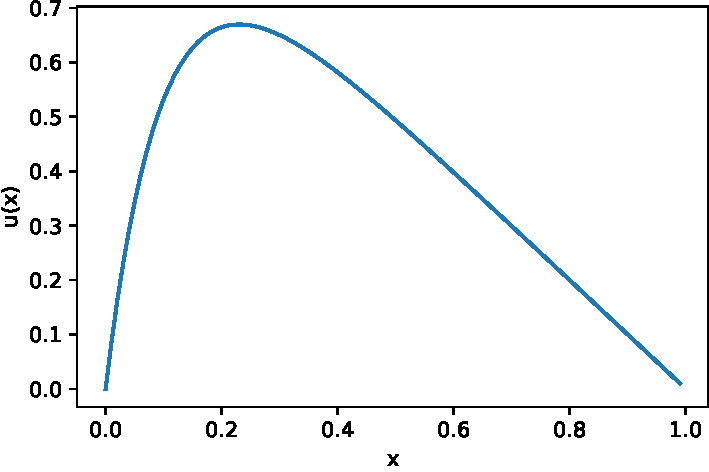
\includegraphics{figs/problem_2.pdf} %Imports the figure.
    \caption{The exact solution $u(x)$ to the Poisson equation with the given source term over its domain.}
    \label{fig:exact}
\end{figure}
%
\section*{Problem 3}
It is well established that an approximation to $u''(x)$ is given as follows:
\begin{equation*}
    u''(x) \approx =  \frac{u(x + h) - 2 u(x) + u(x -h)}{h^2},
\end{equation*}
where $h$ is an appropriately chosen small step-size. For the problem at hand, we are interested in approximating $u''$ over the unit interval.
We define $x_i = i / N$, discretizing the unit interval into $N$ non-overlapping intervals, and let $i = 0 \ldots N$. Furthermore, we 
introduce $u(x_i) = u_i$, and $f(x_i) = f_i$.

Thus, from the original Poisson equation, we can write 
\begin{eqnarray*}
     - \frac{u_{i+1} - 2 u_i + u_{i-1}}{h^2} + \mbox{higher order terms}  & = & f_i, \quad i = 1,\ldots N-1. \\
\end{eqnarray*}
This leads to the simple discrete approximation $v_i$:
\begin{equation*}
    - (v_{i+1} - 2 v_i + v_{i-1})  = h^2 f_i, \quad i = 1,\ldots N-1. 
\end{equation*}
Here, $v_0 = u_0 = u(0) = 0$, $v_N = u_N = u(1) = 0$, and $h = 1/N$. This is the discrete version of the original Poisson equation, 
and if this is solvable (it is!), we have found approximation to $u(x)$ on the discrete grid $x_i$.
%
\section*{Problem 4}
The discrete equation above can be written as follows for $i = 2,\ldots,N-2$:
\begin{equation*}
    \begin{bmatrix}
        -1 & 2 & -1
    \end{bmatrix} 
    \begin{bmatrix}
        v_{i-1}\\v_{i}\\v_{i+1}
    \end{bmatrix}
    = h^2 f_i.
\end{equation*}
However, we need to take care for the cases $i=1$ and $i=N-1$:

\begin{equation*}
    \begin{bmatrix}
    2 & -1
    \end{bmatrix} 
    \begin{bmatrix}
        v_{i}\\v_{i+1}
    \end{bmatrix} - v_{i-1}
    = h^2 f_i, \quad\text{for $i=1$},
\end{equation*}
and,
\begin{equation*}
    \begin{bmatrix}
    -1 & 2
    \end{bmatrix} 
    \begin{bmatrix}
        v_{i-1}\\v_{i}
    \end{bmatrix} - v_{N+1}
    = h^2 f_i, \quad\text{for $i=N-1$}.
\end{equation*}
Stacking these three equations in matrix form, we get
\begin{equation*}
    \begin{bmatrix}
    2   & -1 & \dots & 0 & 0 \\
    -1  & 2 & -1    & \dots & 0 \\
    0   & -1 &\ddots&\ddots&0\\
    \vdots& \ddots & \ddots & \ddots & 0\\
    0 & \dots& \ddots &  -1 & 2
    \end{bmatrix}_{(N-1)\times(N-1)}
    \begin{bmatrix}
        v_{1}\\\vdots\\\vdots\\\vdots\\v_{N-1}
    \end{bmatrix}_{(N-1)\times 1} 
    - 
    \begin{bmatrix}
        v_{0}\\0\\\vdots\\0 \\v_{N}
    \end{bmatrix}_{(N-1)\times 1}
    = h^2    
    \begin{bmatrix}
        f_{1}\\ \vdots\\\vdots\\\vdots \\f_{N-1}
    \end{bmatrix}_{(N-1)\times 1}.
\end{equation*}

This is what we want; we get 
\begin{equation}
    \mathbf A \vec v = \vec g, \label{eq:Avg}
\end{equation}
where 
\begin{equation}
    g_i = 
    \begin{cases}
        h^2 f_i + v_0 & \text{for $i = 1$}\\
        h^2 f_i       & \text{for $i = 2\ldots N-2$}\\
        h^2 f_i + v_N & \text{for $i = N-1$}
    \end{cases}
\end{equation}
%
%
\section*{Problem 5}
\subsection{Relation $n$ to $m$}
Now, we let $\vec{v^*}$ be a complete solution of the discretized Poisson equation. If we employ $N$ intervals, the full solution need to be specified for $N+1$ values. Hence, if 
$\vec{v^*}$ has length $m$, it is clear that $m=N+1$. As described under Problem 4, the matrix $\mathbf A$ has dimensions $(N-1)\times{N-1}$, which is $n\times n$. Thus, $n = m+2$.
\subsection{Relation $\vec{v^*}$  to $\vec{v}$}
From the discussion  above, it appears that solving~\ref{eq:Avg} gives the \emph{interior solution} of the discrete Poisson equation, i.e. not including the boundary conditions.  

\section*{Problem 6}
OK, now $\mathbf A$ is an $n\times n$ tridiagonal matrix, and we are interested in solving $\mathbf A \vec v = \vec g$ for $\vec v$.
\\
\\
\textbf{a) General algorithm}
\\
A general algorithm follows from standard Gaussian elimination forward for eliminating the subdiagonal $a$, and then solving backwards to find $v$.
This is summarized  here for algorithm \ref{algo:thomas}.
\begin{algorithm}[H]
    \caption{Thomas algorithm (Gaussian elimination applied to tridiagonal matrices) }\label{algo:thomas}
    \begin{algorithmic}
        \Require{$a = \left[a_2, \ldots a_n\right], b = \left[b_1, \ldots b_n\right], c = \left[c_1, \ldots c_{n-1}\right], g = \left[g_1, \ldots g_{n}\right]$ }
        \State Allocate memory $\tilde b = \left[\tilde b_1, \ldots \tilde b_n\right], \tilde g = \left[\tilde g_1, \ldots \tilde g_{n}\right], v = \left[v_1, \ldots v_n\right] $
        \State Initialize new diagonal: $\tilde b_1 = b_1$
        \For{$i =  2, ..., n$} \Comment Repeated $n-1$
            %\State $\tilde a_i = a_i - \frac{a_i}{\tilde b_{i-1}} b_{i-1}$ \Comment This is all zero and included for clarity
            \State $\tilde b_i = b_i - \frac{a_i}{\tilde b_{i-1}} c_{i}$ \Comment FLOP: 4
            \State $\tilde g_i = g_i - \frac{a_i}{\tilde b_{i-1}} \tilde g_{i}$ \Comment FLOP: 4
        \EndFor
        \State $v_n = \frac{\tilde g_n}{\tilde b_{n}}$              
        \For{$i =  n-1, ..., 1$} \Comment Repeated $n-1$
            \State $v_i = \frac{\tilde g_i - c_i v_{i+1}}{\tilde b_{i}} $ \Comment FLOP: 4
        \EndFor
        \Return $v$        
    \end{algorithmic}
\end{algorithm}
\textbf{b) Number of FLOPs}
\\
From the algorithm above, we see that the number of FLOPS equals $(n-1)\times(4 + 4) + 1 + (n-1)\times 4 = 12 \times (n-1) + 1$. In other words, solving a triangular system of $n$ linear equations is requires $\approx 12 n$ FLOPs.


\end{document}

